% !TEX root = MSTAT19.tex
% This work is licensed under the Creative Commons
% Attribution-NonCommercial-ShareAlike 4.0 International License. To view a copy
% of this license, visit http://creativecommons.org/licenses/by-nc-sa/4.0/ or
% send a letter to Creative Commons, PO Box 1866, Mountain View, CA 94042, USA.

\subsection{Anwendung von Donsker in der Statistik} \label{sec:donskeranwendung}
\begin{notation}
	Sei $X$ eine reelle Zufallsvariable. Dann schreibe
	\begin{align*}
		X\sim(μ,σ^2):⇔\Earg{X}=μ\qquad\text{und}\qquad\Var(X)=σ^2
	\end{align*}
\end{notation}

Wir betrachten das \define{Change-Point-Problem:}
% mit diesem Problem hat Ferger seine Uni-Karriere gestartet
$X_{1,n},…,X_{n,n},n∈ℕ$%
\footnote{Es wäre sinnvoller, die Indices wie bei Matrizen $X_{n, i}$ zu nummerieren, aber das tut Prof.\ Ferger hier bewusst nicht.}
unabhängig mit
\begin{align*}
	\begin{cases}
		X_{i,n} \text{ \iid} \sim(μ,σ^2), &\falls 1 ≤ i ≤ τ_n\\
		X_{i,n} \text{ \iid} \sim(ν,τ^2), &\falls τ_n < i ≤ n
	\end{cases}
\end{align*}
wobei $τ_n ∈ \set{1,…,n}$ (deterministisch und) \emph{unbekannt}
ist (der sogenannte \define{Change-point (moment of change)})
der Folge $(X_{i, n})_{1 ≤ i ≤ n}$, $n ∈ ℕ$.
% Schreibe kurz $X_i \equiv X_{i, n}$. in den Vorlesungsanschriften

\begin{align*}
	\underbrace{X_{1,n}, …, X_{τ_n,n}}_{\text{\iid\ } \sim(μ,σ^2)}
	\qquad \underbrace{X_{τ_n + 1, n}, …, X_{n,n}}_{\text{\iid} \sim(ν,τ^2)}
\end{align*}
\subparagraph{Annahmen (zunächst):} $μ,σ^2$ bekannt, $ν,τ^2$ unbekannt, $ν>μ$

Das Problem kommt aus der Qualitätskontrolle.
Die Leute beobachten ein Produktionsprozess, z.\,B.\ für Schrauben.
Diese Schrauben brauchen einen bestimmten Durchmesser. Man macht Stichproben.
So lange der Durchmesser $μ$ ist, ist alles \enquote{in Control}.
Dann passiert irgendwas in der Maschine nach einem unbekannten Zeitpunkt
und der Prozess geht \enquote{out of control}.
Diesen Zeitpunkt möchte man a posteriori (im Nachhinein) feststellen
um zu sehen, was man entsorgen muss und das Problem erkennen kann.
Außerdem möchte man während der Produktion diesen Fehler erkennen.

\subparagraph{Ziel:} Finde Test für
$H_0:τ_n=n$, d.\,h.\ es hat kein Wechsel stattgefunden vs.\ $H_1:1≤τ_n<n$, d.\,h.\ es findet
ein Wechsel statt. Außerdem möchten wir die Fehlerwahrscheinlichkeiten (1.\ Art) kontrollieren.
Dazu betrachte
\begin{align*}
	S_k := S_{k,n}
	&:= \frac1{√n} \sum_{i=1}^k \underbrace{\frac{X_{i,n} - μ}{σ}}_{=: ξ_{i,n}}
	&∀\,& 0 ≤ k ≤ n \\
	\Earg{S_k} &= 0 \qquad &∀\,& 0 ≤ k ≤ τ_n
	\intertext{Da}
	S_k &= S_{τ_n} + \frac1{√n} \sum_{i = τ_n + 1}^k \frac{X_{i, n} - μ}{σ} &∀\, & τ_n < k ≤  n
	\intertext{folgt}
	\Earg{S_k}
	&= 0 + \frac1{√n} \sum_{i = τ_n + 1}^k \frac{\overbrace{\Earg{X_{i, n}}}^{= ν} - μ}{σ}
	= \frac1{√n} \klammern[\big]{k-τ_n} \frac{ν - μ}{σ} &∀\,& τ_n < k ≤ n
\end{align*}
%TODO 3x Plots einfügen
% 1. Plot von $(k,\Earg{S_k)}$ einfügen: für k≤τ_n ist es immer 0, für k>τ_n wächst es monoton und liear
% 2.Plot von $(k,S_k)$ einfügen: unter H_1: für k≤τ_n ist es ein "rumzappeln" um die X-Achse; für k>τ_n gibt es dann einen "Drift" nach oben
% 3. Plot von $(k,S_k)$ einfügen, unter H_0: hier kein Drift nach oben, nur herumzappeln um die x_Achse

Plausibler Test:
$H_0$ verwerfen $:⇔ T_n:=\max_{0≤ k≤ n} S_k>k_α$.%
\footnote{$α \ll 1$ steht für den Fehler 1.\ Art. $k_{α}$ soll % \ll = <<
	so gewählt werden, dass die Wahrscheinlichkeit, dass ich $H_0$
	verwerfe unter der Bedingung, dass $H_0$ gilt, maximal $α$ ist:
	$\P_{H_0}(H_0 \text{ verworfen}) ≤ α$.
	Allerdings geht das hier nicht für $n$, aber asymptotisch für $n → ∞$.}

Ein anderer plausibler Test wäre, nur $S_n$ zu betrachten.
Vermutlich hat der aber eine schlechtere Güte.%
\footnote{Das zu überprüfen könnte eine Bachelorarbeit füllen.}%
%
\paragraph{Ziel:} Bestimme \define{kritischen Wert} $k_α$ zu vorgegebenen \define{Signifikanzniveau} $α ∈ \intervallO01$.
%
\begin{lemma}\label{lemma7.17}
	Sei $\ul{y}=\klammern[\big]{y_0,y_1,…,y_n}∈ℝ^{n+1}$ und $h(\ul{y})$ der Polygonzug durch die Punkte $\klammern{\frac{k}{n},y_k}_{0≤ k≤ n}$.
	% CHECKED: '\ul' used.
	Dann gilt:
	\begin{enumerate}[label=(\arabic*)]
		\item \label{it:7.17max} $\begin{aligned}
			\max_{0 ≤ k ≤ n} y_k = \max_{0 ≤ t ≤ 1} h(\ul{y})(t) = \sup_{0 ≤ t ≤ 1} h(\ul{y})(t)
			% CHECKED: '\ul' used.
			\end{aligned}$
		\item \label{it:7.17maxabs} $\begin{aligned}
				\max_{0 ≤ k ≤ n} \abs{y_k} = \max_{0 ≤ t ≤ 1} \abs{h(\ul{y})(t)}
				% CHECKED: '\ul' used.
				= \sup_{0 ≤ t ≤ 1} \abs{h(\ul{y})(t)}
			% CHECKED: '\ul' used.
			\end{aligned}$
		\item \label{it:7.17add} $\begin{aligned}
			\ul{y},\ul{z}∈ℝ^{n+1}, α, β ∈ ℝ ⇒ h\klammern[\big]{α\ul{y} + β\ul{z}} = α h\klammern[\big]{\ul{y}} + β h\klammern[\big]{\ul{z}}
			% CHECKED: '\ul' used.
		\end{aligned}$
	\end{enumerate}
\end{lemma}

\begin{proof} Zur Übung über den Jahreswechsel. Hier eine Lösung:
	\paragraph{Zeige \ref{it:7.17max}:}
	Gemäß der Zwei-Punkte-Formel gilt:
	\begin{align}\label{eqProof7.17Stern}\tag{$\ast$}
		h\klammern[\big]{\ul{y}}(t)
		% CHECKED: '\ul' used.
		&=y_{k-1}+\klammern[\big]{n· t-(k-1)}·\klammern[\big]{y_k-y_{k-1}}
		\qquad∀ t∈\intervall{\frac{k-1}{n}}{\frac{k}{n}}, ∀ 1≤ k≤ n
	\end{align}
	Da
	\begin{align*}
		h\klammern[\big]{\ul{y}}\klammern{\frac{k}{n}}\overset{\text{Def}}{=}y_k\qquad∀ 0≤ k≤ n
		% CHECKED: '\ul' used.
	\end{align*}
	gilt in \ref{it:7.17max} und \ref{it:7.17maxabs} in jedem Fall \enquote{$≤$}. Umgekehrt sei $t∈\intervall01$ beliebig. Dann:
	\begin{align*}
		∃ 1≤ k≤ n:t∈ \intervall{\frac{k-1}{n}}{\frac{k}{n}}
	\end{align*}
	\subparagraph{Fall 1: $y_k ≥ y_{k-1}$}
	Dann ist $h\klammern[\big]{\ul{y}}$ monoton wachsend auf $\intervall{\frac{k-1}{n}}{\frac{k}{n}}$ und es gilt
	% CHECKED: '\ul' used.
	\begin{align*}
		h\klammern[\big]{\ul{y}}(t)≤ h\klammern[\big]{\ul{y}}\klammern{\frac{k}{n}}=y_k≤\max_{0≤ k≤ n} y_k
		% CHECKED: '\ul' used.
	\end{align*}
	\subparagraph{Fall 2: $y_k<y_{k-1}$}
	Dann ist $h\klammern[\big]{\ul{y}}$ monoton fallend und es gilt
	% CHECKED: '\ul' used.
	\begin{align*}
		h\klammern[\big]{\ul{y}}(t)≤ h\klammern[\big]{\ul{y}}\klammern{\frac{k-1}{n}}=y_{k-1}≤\max_{0≤ k≤ n}y_k
		% CHECKED: '\ul' used.
	\end{align*}

	\paragraph{Zeige \ref{it:7.17maxabs}:} In Fall 1 gilt:
	\begin{align*}
		h\klammern[\big]{\ul{y}}(t) & ≤ y_k ≤ \abs{y_k} ≤ \max_{0 ≤ k ≤ n} \abs{y_k}\\
		% CHECKED: '\ul' used.
		h\klammern[\big]{\ul{y}}(t) & ≥ y_{k-1} ≥ -\abs{y_{k-1}} ≥ -\max_{0 ≤ k ≤ n} \abs{y_k}\\
		% CHECKED: '\ul' used.
		⇒
		\abs[\Big]{h\klammern[\big]{\ul{y}}(t)} & ≤ \max_{ 0≤ k ≤ n} \abs{y_k}
		% CHECKED: '\ul' used.
	\end{align*}
	Fall 2 analog. Somit folgt \ref{it:7.17maxabs}.
	\paragraph{Zeige \ref{it:7.17add}:}
	Folgt aus \eqref{eqProof7.17Stern}.
\end{proof}

Es folgt aus dem Lemma \ref{lemma7.17} \ref{it:7.17max} (mit $y_k=S_k$):
\begin{align*}
	T_n &:= \max_{0 ≤ k ≤ n} S_k
	\overset{\ref{lemma7.17}}=
	\max_{0≤ t≤ 1}%\underbrace{
	h\klammern[\big]{S_0,…,S_n}%}_{\overset{\text{Def}}{=}X_n=\text{ Partialsummenproz.}}
	(t)
\end{align*}
Aber $Y_n := h(S_0, ..., S_n)$ ist der Partialsummenprozess zur Folge $\klammern{\frac{X_{i, n} - μ}{σ}}_{1 ≤ i ≤ n} = (ξ_{i, n})_{1 ≤ i ≤ n}$, $n ∈ ℕ$.
\begin{align*}
	T_n
	&=\sup_{0≤ t≤ 1} Y_n(t) = M(Y_n) = M ∘ Y_n, \text{ wobei} \\
	M &\colon C\klammern[\big]{\intervall01} ⟶ ℝ, \qquad M(f) := \sup_{0 ≤ t ≤ 1} f(t),
	\qquad ∀ f ∈ C\klammern[\big]{\intervall01}
\end{align*}
Da
\begin{align*}
	\abs{M(f)-M(g)} \overset{(!)}{≤} \sup_{0 ≤ t ≤ 1} \abs{f(t)-g(t)} = d(f,g)
\end{align*}
ist $M$ stetig auf $C\klammern[\big]{[0,1]}$ folgt mit Dreiecksschematabemerkung zu Donsker \ref{bemerkung7.16Einhalb} und dem CMT \ref{satz4.10ContinuousMappingTheorem}:
\begin{align*}
	T_n=M(X_n)\distrto  M(B)=\sup_{0≤ t≤ 1} B(t),~\text{\emph{falls} $H_0$ gilt}
\end{align*}
Funktionale auf der Brownschen Bewegung sind gut untersucht.
Es gilt (siehe %z.\,B.\ Borodin + Salminen)
\cite{borodin2012handbook}):
\begin{align*}
	\sup_{0≤ t≤ 1}B(t)
	\overset{\L}&=
	\abs{\mathcal{N}(0,1)} \quad \klammern[\Big]{=\abs{Z},~ Z \sim \mathcal{N}(0,1)} \\
	⇒
	\underbrace{
	\P_{H_0}\argu[\big]{T_n > k_{α}}
	}_{=1-\P\argu[\big]{T_n ≤ k_{α}}}
	&\ntoinf \P\argu[\big]{\abs{Z} > k_{α}}
	= 1 - \P\argu[\big]{\abs{Z} ≤ k_{α}},% \qquad ∀ x ∈ ℝ,
\end{align*}
da Verteilungsfunktion $Φ$ von $\abs{Z}$ stetig auf ganz $ℝ$, denn:
\begin{align*}
	\P\klammern[\big]{\abs{Z} > k_{α}}
	\stackrelnew{Z \stackeq{\L} -Z}{\text{Sym}}{=}
	2 \klammern[\big]{1-Φ(k_{α})}
\end{align*}
Also folgt
\begin{align*}
	\P\argu[\big]{T_n>k_α} \ntoinf 2 \klammern[\big]{1 - Φ(k_α)} \stackeq{!}α \\
	2 \klammern[\big]{1 - Φ(k_α)} = α
	⇔ 1-\frac{α}{2}=Φ(k_α)\\
	⇔ k_α=Φ^{-1}\argu{1-\frac{α}{2}} =: u_{1 - \frac{α}{2}}
\end{align*}
Es folgt: Der Test \enquote{$H_0$ verwerfen $:⇔ T_n> u_{1-\frac{α}{2}}$} %α/2-Quantil der Standardnormalverteilung
ist ein \define{asymptotischer Niveau-$α$-Test für $H_0$}, d.\,h.
\begin{align*}
	\limn\P_{H_0}\argu[\big]{H_0\text{ wird verworfen}} = α \qquad ∀ α ∈ (0,1)
\end{align*}

Falls nur bekannt, dass $ν\neqμ$, so modifiziere obigen Test zu
\begin{equation} \tag{+} \label{eq:7TestBetrag}
	H_0 \text{ verwerfen } :⇔ \hat{T}_n := \max_{0 ≤ k ≤ n} \abs{S_k} > c_α
\end{equation}
Aus \ref{lemma7.17} \ref{it:7.17maxabs} folgt:
\begin{align*}
	\hat{T}_n = \sup_{0 ≤ t ≤ 1} \abs{X_n(t)} = \norm{ X_n}_∞ =: \hat{M}(X_n)
\end{align*}
Da $\hat{M}$ stetig auf $C\klammern[\big]{[0,1]}$ ist, folgt analog wie oben mit dem \ref{it:4.10CMThcontinous} und Donsker \ref{bemerkung7.16Einhalb}
\begin{equation} \tag{$*$} \label{eq:7TestKonvergenzZuBB}
	\hat{T}_n = \hat{M}(X_n) \distrto \hat{M}(B) = \sup_{0 ≤ t ≤ 1} \abs{B(t)} \text{ unter $H_0$}
\end{equation}
Es gilt (vergleiche \cite{shorack2009empirical}):% z.\,B.\ Shorak und Wellner (1986) \undefine{Empirical Processes with applications to statistics}):
\begin{align*}
	H(x):&=\P\klammern{\sup_{0≤ t≤ 1} \abs{B(t)}≤ x}
	=
	\begin{cases}
		\frac{4}{π} \sum_{k ∈ ℕ_0} \frac{(-1)^k}{2k + 1} \exp\argu{-\frac{(2k + 1)^2 π^2}{8· x^2}}, &\falls x>0\\
			0, & \falls x ≤ 0
	\end{cases}
\end{align*}
Ferner ist $H$ stetig auf $ℝ$ und streng monoton wachsend auf $(0,∞)$. Somit erhalten wir (analog wie oben)
\begin{align*}
	\P_{H_0}(\hat T_n > c_{α}) &= 1 - \P_{H_0}(\hat T_n \leq c_{α}) \ntoinf \P( \norm{B}_{∞} \leq c_{α}) & \text{wg.\ \eqref{eq:7TestKonvergenzZuBB} und \ref{korollar4.5}} \\
	⇒ 1 - H(c_{α}) &= 1 - H(H^{-1}(1-α)) = α \\
	\limn\P_{H_0} (H_0\text{ wird verworfen}) &= α & ∀ α ∈ \intervallO01
\end{align*}
\emph{falls} man $c_α:=H^{-1}(1-α)$ wählt.
Das heißt unser Test in \eqref{eq:7TestBetrag} ein asymptotischer Niveau-$α$-Test für $H_0$.

Natürlich ist die Annahme $μ$ und $σ^2$ beide bekannt sehr restriktiv.
Falls beide Parameter unbekannt, so ersetze sie durch Schätzer (sogenannte \define{Substitutionsmethode} bzw.\ \define{Plug-in-method}).
\begin{align*}
	\overline{X}_n := \frac1n \sum_{i=1}^n X_i,\qquad
	\hat{σ}_n^2 := \frac1n \sum_{i=1}^n \klammern[\big]{X_i - \overline{X}_n}^2
\end{align*}
Wir wissen
\begin{align*}
	\klammern[\big]{\overline{X}_n,\hat{σ}_n^2}
	\ntoinf \klammern[\big]{μ,σ^2}\qquad\P_{H_0}\text{-f.\,s.}
\end{align*}
Beachte: Es gibt auch ein starkes Gesetz der großen Zahlen (SGGZ bzw.\ auf englisch SLLN) für Dreiecksschemata (arrays),
% CHECKED: 'bzw.' used.
siehe \cite{chow1997probability}.% z.\,B.\ Chow und Teicher (1997) \undefine{Probability Theory - Independence, Interchangeability, Martingales}

Das Ersetzen von $μ$ und $σ^2$ in der Statistik
\begin{align*}
	T_n = \max_{0 ≤ k ≤ n} \frac1{√n} \abs{\sum_{i=1}^k \frac{X_i-μ}{σ}}
\end{align*}
liefert die \define{Teststatistik} (oder \define{Prüfgröße}).
\begin{align*}
	T_n^\ast
	:&= \frac1{\hat{σ}_n} \frac1{√n} \max_{0 ≤ k ≤ n} \abs{\sum_{i=1}^k\klammern[\big]{X_{i,n} - \overline{X}_n}}
	\mit \hat{σ}=√{\hat{σ}^2}
\end{align*}

\begin{satz}\label{satz7.18}
	Unter $H_0$ gilt:
	\begin{align*}
		T_n^\ast \distrto \sup_{0≤ t≤ 1}\abs[\big]{B(t) - t B(1)}, \quad n → ∞
	\end{align*}
\end{satz}

\begin{proof}
	\begin{align*}
		X_i-\overline{X}_n
		&= X_i - \frac{1}{n} \sum_{j=1}^n X_j
		=σ · \klammern[\bigg]{ % here · to make clear that sigma is not a function but a factor
			\underbrace{\frac{X_i-μ}{σ}}_{=:Z_i}
			-\underbrace{\frac1n \sum_{j=1}^n \frac{X_j-μ}{σ}}_{=:\overline{Z}_n}} \\
		⇒
		T_n^\ast
		&= \frac{σ}{\hat{σ}_n} \max_{0 ≤ k ≤ n} \abs{
			\frac1{√n} \sum_{i=1}^k \klammern[\big]{Z_i-\overline{Z}_n}
		}
		= \frac{σ}{\hat{σ}_n} \max_{0 ≤ k ≤ n} \abs{
		\frac1{√n} \sum_{i=1}^k Z_i - \frac1{√n}k\frac1n \sum_{i = 1}^n Z_i
		} \\
		&= \frac{σ}{\hat{σ}_n} \max_{0 ≤ k ≤ n} \abs{S_k - \frac kn S_n}\\
		\overset{\ref{lemma7.17} \ref{it:7.17maxabs} + \ref{it:7.17add}}&=
		\frac{σ}{\hat{σ}_n} \max_{0 ≤ t ≤ 1} \abs[\Big]{\underbrace{X_n(t) - t X_n(1)}_{=: Y_n(t)}}
	\end{align*}
	wobei $X_n$ der Partialsummenprozess zu $Z_1,…,Z_n$ ist (= Polygonzug durch $\klammern{\frac{k}{n},S_k}$)\footnote{Achtung! Hier ist das $X_n$ etwas anderes als das $X_i$ am Anfang des Beweises: $X_i$ ist eine Kurzschreibweise für $X_{in}$ und $X_n$ der beschriebene Polygonzug!} und
	$S_k:=\frac{1}{√{n}} \sum_{i=1}^k Z_i$.

	Betrachte die Abbildung
	\begin{align*}
		&h \colon C\klammern[\big]{ \intervall01} ⟶ C\klammern[\big]{[0,1]},
		\qquad f ↦ h(f) \colon \intervall01 ⟶ ℝ, \qquad t ↦ h(f)(t) := f(t) - t f(1) \\
		&⇒ Y_n = h(X_n)
	\end{align*}
	Wir zeigen nun, dass $h$ stetig ist.
	\begin{align*}
		\abs{h(f)(t)-h(g)(t)}
		&= \abs{f(t)-t· f(1)-\klammern[\big]{g(t)-t· g(1)}}\\
		&= \abs{f(t)-g(t)-t · \klammern[\big]{f(1)-g(1)}}\\
		\overset{\text{DU}}&{≤}
		\abs{f(t)-g(t)} + \underbrace{\abs{t}}_{≤ 1} \abs{f(1)-g(1)}\\
		&≤
		2 d(f,g) \qquad ∀ t ∈ \intervall01 \\
		⇒ d\klammern[\big]{h(f),h(g)} & ≤ 2 d(f,g) \qquad ∀ f, g ∈ C\klammern[\big]{\intervall01}
	\end{align*}
	Also ist $h$ stetig auf $C\klammern[\big]{[0,1]}$. Dann folgt aus Bemerkung  \ref{bemerkung7.16Einhalb} + CMT \ref{satz4.10ContinuousMappingTheorem}:
	\begin{align*}
		Y_n=h(X_n)\distrto  h(B)=:B_0\text{ in }C\klammern[\big]{[0,1]}
	\end{align*}
	wobei $B_0(t) \overset{\text{Def}}{=} B(t) - t B(1)$.
	\begin{align*}
		\sup_{0≤ t≤ 1} \abs{Y_n(t)} = \hat{M}(Y_n)=\norm{ Y_n}_∞
		\stackrelnew{\ref{satz4.10ContinuousMappingTheorem}}{\L}{\longrightarrow}
		\norm{ B_0} = \sup_{0≤ t≤ 1} \abs{B_0(t)}
	\end{align*}
	Da $\frac{σ}{\hat{σ}_n}\stochto1$, liefert \ref{beisp4.18} \ref{it:4.18einDim}:
	\begin{equation*}
		T_n^\ast = \frac{\sigma}{\hat{\sigma}_n} \norm{Y_n}_{∞}
		\distrto \sup_{0≤ t≤ 1} \abs{B_0(t)} = \norm{B_0}_{∞}
		\qedhere
	\end{equation*}
\end{proof}

\begin{definition} %7.19
	Sei $B$ ein Brownsche Bewegung auf $[0,1]$. Der stochastische Prozess
	\begin{align*}
		B_0(t) := B(t) - t B(1) \qquad ∀ t ∈ \intervall01
	\end{align*}
	heißt \define{Brownsche Brücke}.
	Klar: $B_0$ ist ein stetiger stochastischer Prozess.
\end{definition}

\begin{figure}[H]
	\begin{center}
		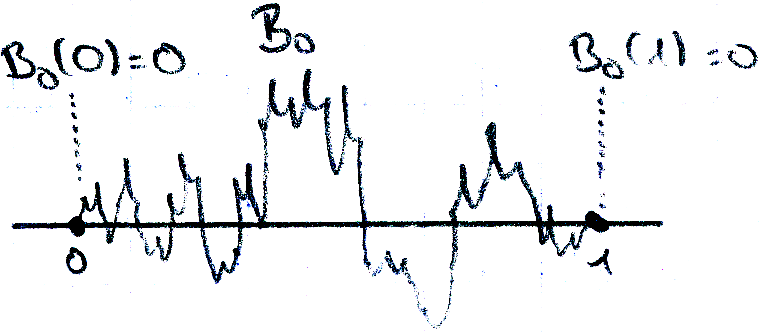
\includegraphics[width=1\textwidth]{./pics/MSTAT002.png}
		\caption{Brownsche Brücke}
		\label{AbbBrownscheBruecke}
	\end{center}
\end{figure}
%Ferger: „Brücke ist doch so'n Ding, da geht man rüber über den Fluss.“
%Ferger: "Also über die Brücke würde ich jetzt nicht gehen. Kein Ahnung, warum man Brücke dazu sagt." → dieses Jahr hat er eine "super" Deutung: ein Charakteristikum einer Brücke
% ist, dass man bei Niveau losgeht und wieder bei Niveau 0 ankommt.

%T_n^\ast ist Supremumsnorm von Partialsummenprozess?+

Es gilt (vergleiche \cite[Seite 34]{shorack2009empirical}%Shorak und Wellner 1986 \undefine{empirical processes}, Seite 34)
\begin{align*}
	H_0(x) &:= \P \argu{\sup_{0 ≤ t ≤ 1} \abs{B_0(t)} ≤ x}
	\overset{\text{Doob}}{=}
	% Doob war ein Mathematiker, der das ausgerechnet hat
	1 - \sum_{k≥ 1}(-1)^{k+1} \exp\argu{-2 k^2 x^2} & ∀ x > 0 \\
	H_0(x) &~= 0 & ∀ x ≤ 0
\end{align*}
$H_0$ ist stetig auf $ℝ$ und streng monoton auf $\intervallHO0{∞}$.
Folglich ist der Test
% für uns: Details wie oben ergänzen
\begin{align*}
	H_0\text{ verwerfen }:⇔ T_n^\ast>H_0^{-1}(1-α)
\end{align*}
ein asymptotischer Niveau-$α$-Test, d.\,h.
\begin{equation*}
	\P_{H_0}(\text{$H_0$ wird verworfen}) = \P_{H_0}(T_n^* > H_0^{-1}(1-α)) \ntoinf α
\end{equation*}
Die Quantilfunktion $H_0^{-1}$ ist in Computerprogrammpaketen implementiert,
z.\,B.\ in MATHEMATICA.
$H_0$ ist die Verteilungsfunktion der \define{Kolmogorov-Smirnov-Verteilung}.

Falls $μ,σ^2$ unbekannt, aber $ν>μ$, so betrachte
\begin{align*}
	\tilde{T}_n&:=\frac1{√n \hat{σ}_n} \max_{0 ≤ k ≤ n} \klammern{\sum_{i=1}^k X_i - \overline{X}_n}
\end{align*}
Vollkommen analog folgt: $\tilde{T}_n\distrto \sup_{0≤ t≤ 1} B_0(t)$ unter $H_0$.
% Beträge in T_n^* kommt von Unwissen, was von ν und μ größer ist, wenn man das weiß, dass ν > μ, so fallen nur die Beträge weg
% folgende Zeilen wurden WiSe 2019/20 dann weggelassen aus Zeitgründen: (bis "Anstelle")
Es gilt (vergleiche z.\,B.\ \cite[Seite 322]{gaensslerstute1977Wahrscheinlichkeitstheorie}%Gänssler + Stute (1977) \undefine{Wahrscheinlichkeitstheorie}, Seite 322)
\begin{align*}
	H_0^+(x) &:= \P\argu{\sup_{0≤ t≤ 1} B_0(t) ≤ x} = 1 - \exp\argu{-2 x^2} & ∀ x ≥ 0 \\
	H_0^+(x) &:= 0 & ∀ x < 0
\end{align*}
Da
\begin{align*}
	(H_0^+)^{-1}(1-α)&=\klammern{-\frac{1}{2}·\log(α)}^{\frac{1}{2}}
\end{align*}
folgt, dass der (einseitige) Test
\begin{align*}
	H_0\text{ verwerfen}:⇔\tilde{T}_n>\klammern{-\frac{1}{2}·\log(α)}^{\frac{1}{2}}
\end{align*}
ein asymptotischer Niveau-$α$-Test für $H_0$ ist.

Anstelle von
\begin{align*}
	T_n^\ast = \frac1{√n \hat{σ}_n} \max_{0≤ k ≤ n}
	\abs[\bigg]{\underbrace{\sum_{i=1}^k \klammern[\big]{X_i - \overline{X}_n}}_{=: C_k}}
\end{align*}
(die $C_k$ heißen \define{kumulierte Summe}) betrachtet \cite{csorgo1997limit} %Csörgő und Horváth (1977) in \undefine{Limit Theorems in Change-point Analysis}
\emph{gewichtete} kumulierte Summen:
\begin{align*}
	U_n^\ast &:= √{n} \frac{1}{\hat{σ}_n} \max_{1≤ k≤ n-1} \frac{\abs{C_k}}{√{k (n - k)}}
\end{align*}

\begin{thm}[Csörgő und Horváth]\label{theoremCH} %noNumber
	Seien
	\begin{align*}
		A_n &:= √{2 \log\argu[\big]{\log(n)}}\\
		D_n &:= 2 \log\argu[\big]{\log(n)} + \frac12 \log\argu[\Big]{\log\argu[\big]{\log(n)}} - \frac12 \log(π) % \qquad ∀ n ≥ n_0 % keine Ahnung, was das soll
	\end{align*}
	Dann gilt unter $H_0$:
	\begin{align}\label{eqTheoremCsorgoHorvath}\tag{1}
		\limn \P_{H_0} \argu[\Big]{A_n U_n^\ast - D_n ≤ t} = \exp\argu[\big]{-2 \exp(-t)} = e^{-2 e^{-t}} =: G(t)
		\qquad ∀ t ∈ ℝ
	\end{align}
	$G$ ist die sogenannte \define{Gumbel-Verteilung}.
\end{thm}

Damit ist die Konstruktion eines asymptotischen Niveau-$α$-Tests für $H_0$ wie folgt möglich: Sei
\begin{align*}
	t_α &:= G^{-1}(1-α) = -\log\argu{-\frac12 \log(1-α)}
\end{align*}
Klarerweise gilt:
\begin{align*}
	A_n U_n^\ast - D_n > t_α ⇔ U_n^\ast > \frac{t_α + D_n}{A_n} := d_n(α)
\end{align*}
Somit ist
\begin{align*}
	H_0\text{ verwerfen}:⇔ U_n^\ast>d_n(α)
\end{align*}
ein asymptotischer Niveau-$α$-Test, d.\,h.
\begin{align}\label{eqUnderTheoremCsorgoHarcath}\tag{2}
	\limn\P_{H_0}\klammern[\big]{U_n^\ast>d_n(α)}
	= \limn \P_{H_0} \argu[\big]{A_n U_n^* - D_n > t_{α}}
	\overset{\eqref{eqTheoremCsorgoHorvath}}{=} 1 - G(t_{α}) = α
\end{align}
\define{Problem:} Die Konvergenz in \eqref{eqTheoremCsorgoHorvath} und damit in \eqref{eqUnderTheoremCsorgoHarcath} ist sehr sehr sehr laaaaaangsaaaam. %genauso stand das an der Tafel
% im 2. Jahr nur das zweite a vervielfacht
% CHECKED: 'bzw.' used.
%Ferger: "[...] Grottenschlecht."
% „n geht gegen ∞, aber das Leben ist endlich“
Andererseits führen die Gewichte in $\klammern[\big]{k (n - k)}^{ -\frac{1}{2} }$ in $U_n^\ast$ zu einer verbesserten Sensitivität (Güte) des \define{$U_n^\ast$-Tests} unter der Alternative ($H_1$), \emph{insbesondere}, falls $τ_n$ nahe bei $1$ oder $n-1$ (\enquote{am Rand}) liegt.
\paragraph{Idee:}% Bei der Bratwurscht. Prof. Ferger hatte diese Idee während eine Bratwurscht in der Pfanne brutzelte.
Weiterhin gewichten, aber durch die einzelne (das heißt von $k$ unabhängige)
und \emph{zufällige} Größe $√{\hat{k}_n (n-\hat{k}_n)}$ wobei
\begin{align*}
	\hat{k}_n &:= \min \set{ 1 ≤ k ≤ n : \abs{C_k} = \max_{1 ≤ j ≤ n-1} \abs{C_j} } \\
						% &= \text{kleinste Maximalstelle des Prozesses $j ↦ C_j$} \\
	C_j &:= \sum_{i=1}^j \klammern[\big]{X_i-\overline{X}_n}
\end{align*}
d.\,h.\ $\hat{k}_n$ ist die kleinste Maximalstelle von $\abs{C_k},k∈\set{1,…,n-1}$. Erhalte:
\begin{align*}
	R_n = \frac{√n}{\hat{σ}_n}
	\frac{\max_{1 ≤ k ≤ n-1} \abs{ \sum_{i=1}^k (X_i-\overline{X}_n) }}{√{\hat{k}_n (n - \hat{k}_n)}}
\end{align*}

\begin{thm}[Dietmar Ferger, 2018, \cite{ferger2018supremum}]%\liabel{theoremFerger2018} %nonumber
	Sei $X_{1n}, ..., X_{nn}$ ein Dreiecksschema von \iid\ Zufallsvariablen mit positiver endlicher Varianz. Dann gilt:
	\begin{align}\label{eqTheoremFerger2018}\tag{3}
		R_n &\distrto R
		\qquad \text{wobei} \qquad
		R = \frac{M}{√{T (1 - T)}} \mit \\
		M &:= \sup_{0 ≤ t ≤ 1} \abs{B_0(t)} \nonumber,\qquad
		T:=\argmax_{0<t<1} \abs{B_0(t)}, \qquad
		B_0=\text{ Brownsche Brücke}\nonumber
	\end{align}
\end{thm}

In diesem Theorem %\ref{theoremFerger2018}
werden Dichte und Verteilungsfunktion $F_R$ von $R$ explizit bestimmt
($F_R$ hat Reihendarstellung).
%Ferger: "Sie müssen immer eine Anwendung haben. Am besten Sie retten die Welt."
Falls $r_α:=F_R^{-1}(1-α)$, so liefert \eqref{eqTheoremFerger2018} für den Test
\begin{align*}
	H_0\text{ verwerfen}:⇔ R_n>r_α
\end{align*}
dass gilt:
\begin{align*}
	\limn\P_{H_0}\klammern[\big]{R_n>r_α}=α
\end{align*}

\begin{bemerkung}
	\eqref{eqTheoremFerger2018} gilt für $X_{1,n},…,X_{n,n}$ \iid\ $∀ n∈ℕ$.\\
	In Monte-Carlo-Simulationen zeigt der $R_n$-Test eine deutlich bessere Güte als der $U_n^\ast$-Test von Csörgő und Horvath.

	Falls bekannt ist, dass $ν>μ$, so betrachte
	\begin{align*}
		R_n^+&:=√{n}·\frac{1}{\hat{σ}_n}·\frac{\max_{1≤ k≤ n-1}\sum_{i=1}^k\klammern[\big]{X_i-\overline{X}_n}}{√{\hat{k}_n^+·\klammern[\big]{n-\hat{k}_n^+}}}\\
		\hat{k}_n^+&:=\min\set{ 1≤ k≤ n-1:C_k=\max_{1≤ j≤ n-1}C_j}
	\end{align*}
\end{bemerkung}
\footnote{Folgendes wurde im Wintersemester 2019/2020 erwähnt:

	Es gilt:
	\begin{align*}
		R_n^+\distrto  R^+=\frac{M^+}{√{T^+·(1-T^+)}},\qquad
		M^+=\sup B_0(t),\qquad
		T^*=\argmax B_0(t)\\
		H^+(x) := \P\argu[\big]{R^+≤ x}
		= 2 Φ(x) - √{\frac2{π}} x \exp\argu{-\frac12 x^2} - 1
		\qquad x ≥ 0 ~ (=0, x<0)
	\end{align*}
	Hierbei ist $Φ$ die Verteilungsfunktion der Standardnormalverteilung. Ferner gilt:
	Die Zufallsgrößen $R^+$ und $T^+$ sind stochastisch unabhängig!
	\begin{align*}
		\hat{τ}_n-τ_n\distrto V &= \\
		% todo: something is missing!
		\hat{τ}_n &:= \argmax_{1≤ k≤ n-1} \abs{\sum_{i=1}^k\klammern[\big]{X_i - \overline{X_n}}}
	\end{align*}
}

